\usecaseristoratore{Visualizzazione lista prenotazioni}
\label{usecase:Visualizzazione lista prenotazioni}

\begin{figure}[h]
	\centering
	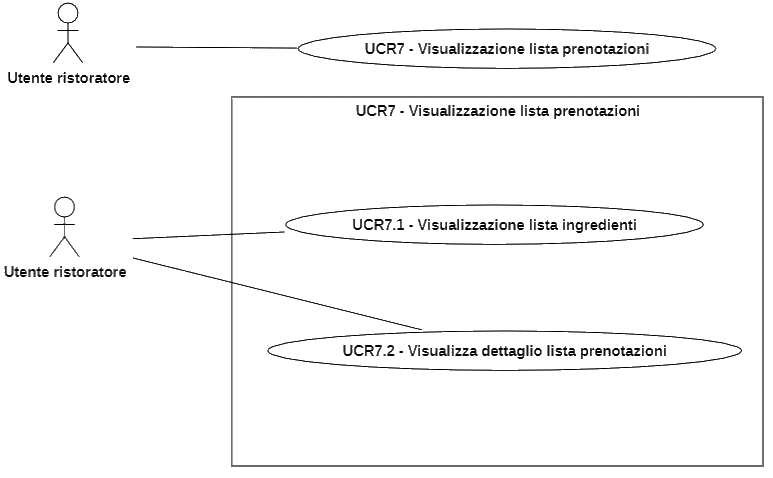
\includegraphics[width=0.7\textwidth]{./uml/UCR7.png} 
	\caption{Visualizzazione lista prenotazioni}
	\label{fig:UCR7}
  \end{figure}

\begin{itemize}
	\item \textbf{Attore principale:} Utente ristoratore.

	\item \textbf{Precondizione:} L'Utente ristoratore ha effettuato l'accesso al Sistema (vedi \autoref{usecase:Effettua accesso}).

	\item \textbf{Postcondizione:} L'Utente ristoratore visualizza la lista di
		prenotazioni (prenotazioni che si trovano in qualsiasi stato) attraverso
		una vista a calendario mensile.

	\item \textbf{Scenario principale:}
	      \begin{enumerate}
		      \item Il Sistema mostra una vista a calendario mensile, in ogni
				  giorno del mese l'utente può consultare:
		            \begin{itemize}
			            \item La lista di prenotazioni.
			            \item La lista di ingredienti con le quantità necessarie 
							per soddisfare la richiesta giornaliera 
							(vedi \autoref{usecase:Consultazione lista ingredienti}).
		            \end{itemize}

		      \item Il Sistema mostra la lista prenotazioni inerente ad un 
				  giorno nei due modi seguenti:
		            \begin{itemize}
			            \item Di \textit{default}, nella lista, le prenotazioni 
							sono mostrate in ordine di orario crescente;

			            \item L'Utente ristoratore può riordinare le 
							prenotazioni, per facilitare la consultazione della 
							lista a seconda dei suoi bisogni, in base a:
							\begin{itemize}
								\item Orario di prenotazione;
								\item Stato della prenotazione;
								\item Numero della prenotazione;
							\end{itemize}
		            \end{itemize}

		      \item L'Utente ristoratore visualizza la lista di prenotazioni a
				  vista giornaliera.
	      \end{enumerate}
\end{itemize}


\subusecaseristoratore{Visualizzazione lista ingredienti}
\label{usecase:Consultazione lista ingredienti}
\begin{itemize}

	\item \textbf{Attore principale:} Utente ristoratore.

	\item \textbf{Precondizione:} L'Utente ristoratore si trova nella sezione 
		"Consultazione lista prenotazioni" (vedi 
		\autoref{usecase:Visualizzazione lista prenotazioni}).

	\item \textbf{Postcondizione:} L'Utente ristoratore visualizza la lista 
		ingredienti aggiornata.

	\item \textbf{Scenario principale:}
	      \begin{enumerate}
		      \item Il Sistema mostra la lista ingredienti necessari per la 
				  giornata (relativamente alle prenotazioni negli stati: "In
				  attesa", "Approvata", "In corso", "Pagamento", "Conclusa");
		      \item L'Utente ristoratore visualizza la lista degli ingredienti.
	      \end{enumerate}

\end{itemize}

\subusecaseristoratore{Visualizza dettaglio lista prenotazioni}
\label{usecase:Visualizza dettaglio lista prenotazioni}
\begin{itemize}
	\item \textbf{Attore principale:} Utente ristoratore.

	\item \textbf{Precondizione:} L'Utente ristoratore ha consultato la lista delle prenotazioni (vedi \autoref{usecase:Visualizzazione lista prenotazioni}).

	\item \textbf{Postcondizione:} L'Utente ristoratore visualizza le prenotazioni in dettaglio.


	\item \textbf{Scenario principale:}
	      \begin{enumerate}
		      \item L'Utente ristoratore seleziona un giorno nel calendario a
				  vista mensile da visualizzare in dettaglio;
		      \item Il Sistema mostra tutte le prenotazioni presenti nel giorno selezionato dall'Utente ristoratore;

		      \item L'Utente ristoratore seleziona una prenotazione da visualizzare in dettaglio;
		      \item Il Sistema mostra i dettagli e le informazioni relative alla prenotazione selezionata dall'Utente ristoratore:
		            \begin{itemize}
			            \item Numero della prenotazione;
			            \item Orario della prenotazione;
			            \item Numero di persone;
						\item Totale della prenotazione (se la prenotazione ha
							qualche ordine associato);
			            \item Stato della prenotazione;
						\item Metodo di divisione del conto;
						\item Numero degli ordini pagati.
		            \end{itemize}
	      \end{enumerate}
\end{itemize}
